\begin{frame}
\frametitle{Higgs Discovery Plot - Use of Monte Carlo Simulation}

\begin{columns}[T] % align columns

\begin{column}{.60\textwidth}
\begin{figure}[htbp]
\begin{center}
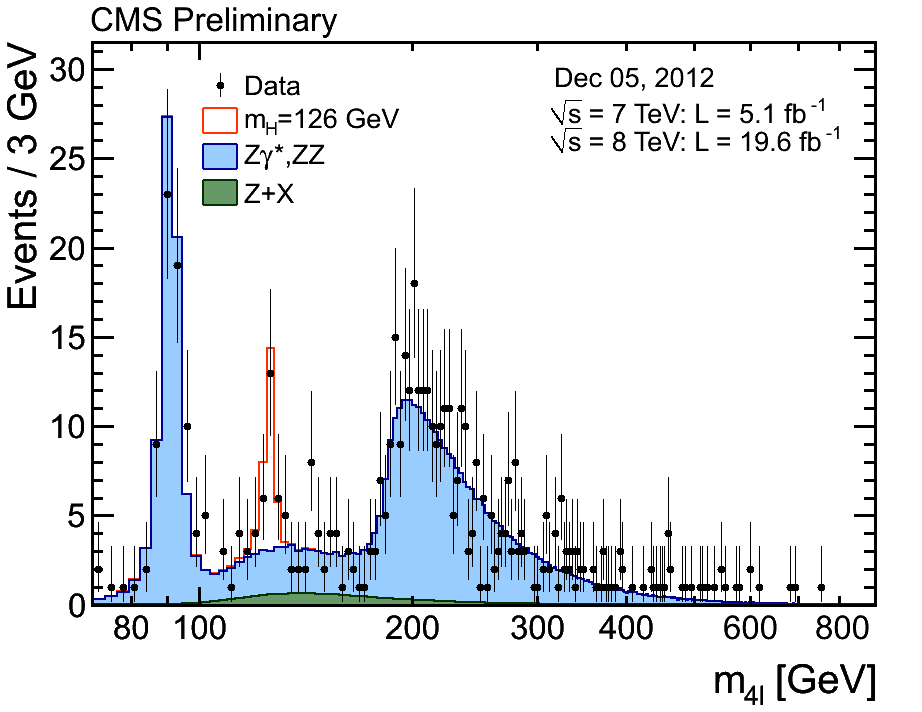
\includegraphics[width=0.95\textwidth]{images/higgs-discovery-plot.png}
%\caption{}
%\label{fig:example2}
\end{center}
\end{figure}
\end{column}%

\begin{column}{.40\textwidth}
\begin{itemize}
\item Detect particle interactions and compare to standard model
\item Black dots (with error bars) are measurements
\item Blue shape: simulation of standard model
\item Red shape: simulation of new theory (in this case the Higgs)
\end{itemize}
\end{column}%

\end{columns}

%\small{Example Text}

\end{frame}


